%a cusomized summary with Latex to to generate yours,  you can add external links to your email , github repo, personal linkedIn profile
\documentclass{my_cv}
\begin{document}

\name{Full NAME}
\contact{City}{Country} {\href{mailto:yourEmail@gmail.com}{yourEmail@gmail.com}}{(+212)-666-6666}


%Small description of who you are

\section{Objective}
\hspace{1pt}\parbox{0.99\textwidth}{
A polyvalent Engineer who has 3 years experience as an automotive/embedded/Web engineer and 
involved in software tests where test cases were developed, automated and 
executed. Experienced in embedded systems’ testing: system test, smoke test, 
regression test, etc. Efficient in working with geographically distributed 
teams (Agility: SCRUM).
}

\vspace{-7pt}

% Education

\section{Education}

\edsubsection{Faculty of Sciences and Technologies}{Settat, Morocco}{Master degree in Embedded Systems and Telecommunication Engineering}{2013--2019}\\
\vspace{3pt}
\edsubsection{Technical high school}{Fez, Morocco}{National High School Diploma, Electrical Sciences and Technologies}{June 2013}
 \\



\vspace{-7pt}
%you can add your linkedIn link profile
\section{Work Experience \hfill  {\small \href{https://www.linkedin.com/feed/}{
\includegraphics[scale=0.075]{LI-Logo.png}}}}

%Here you can add you work experience 
%copy the worksubsection as many as you have experience
\worksubsection{Capgemini Engineering}{Casablanca, Morocco}{Software Engineer}{December 2022 – Now}{Project:}
{Client}{Project description}{
    \item  Task 1
    \item  Task 2
      \item  Task 3




}\vspace{0.1cm}
\worksubsection{Metaneon Maroc}{Fez, Morocco}{Self-employed}{December 2021 – December 2022}{Project:}
{Metaneon}{Making artistic connected neon signs }{
    \item worked on the whole process of the Neon signs creation
    \item Content creation 
    \item Art Direction 
    \item Automation 
   \item Marketing and B2B and B2C support
   \item Instagram :\href{https://www.instagram.com/metaneon_mar/}{\textcolor{blue}{\underline{Metaneon\_mar}}}


}\vspace{0.1cm}



\vspace{-12pt}

% Here you can add your skills
\section{Skills}
\begin{itemize}[leftmargin=10pt, itemsep=0pt]

\item {\bf Languages}: C, CAPL, Python, REST, ASAM OpenDrive
\item {\bf Tools}: Canoe, vTESTstudio, Matlab\textbackslash Simulink,IPG Car Maker, ECU-TEST, INCA, TRACE32, DLT viewer
\item {\bf  OSes}:  Linux (Embedded), Windows
\item {\bf  Protocols}:  CAN, Ethernet, UDS, XCP, Flexray, LIN
\item {\bf Documentation}:  IBM DOORS, RQM, Polarion
\item {\bf  Defect Management}: JIRA, IBM RTC Jazz
\item {\bf   Version Control}: GIT, SVN
\item {\bf Standards}:  ISO-26262, MISRA-C
\item {\bf Methodologies}:  A-SPICE v3, AUTOSAR, OOP, V-Model, Agile (SCRUM)


\end{itemize}

%Academic projects are here and a link to your experiences in LinkedIn
\section{Academic Projects  \hfill  {\small \href{https://www.linkedin.com/in/hamid-tasra-943700126/details/experience/}{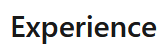
\includegraphics[scale=0.75]{Capture.png}}}}


\begin{itemize}[leftmargin=10pt, itemsep=0pt]
\item {\bf Safe Drive}:  Backpack used by Cyclists to prevent them against road accidents
\begin{itemize}\vspace{-8pt}
\item {\bf Tools}: C, Atmel® ATmega328P, PIC16F877A, MPU6050, RF 433MHz, RGB Panel
\end{itemize}
\vspace{-4pt}
\item {\bf Smart Headlight}: Automatic control of car headlights  
\begin{itemize}\vspace{-8pt}
\item {\bf Tools}: Python, MQTT, Raspberry Pi, Embedded Linux, ESP8266, PiCamera
\end{itemize}
\vspace{-4pt}
\item {\bf Home automation}: Prototype of a smart home for devices monitor using a web application
\begin{itemize}\vspace{-8pt}
\item {\bf Tools}: Raspberry Pi, LAMP, HTML, CSS, SQL, PHP, DS18B20, PiCamera
\end{itemize}
\end{itemize}

%Certifications

\section{Certification}
	
\begin{itemize}[leftmargin=10pt, itemsep=0pt]
    \item ISTQB certified tester foundation level - \href{http://scr.istqb.org/?name=tasra&number=81569&orderBy=relevancy&orderDirection=&dateStart=&dateEnd=&expiryStart=&expiryEnd=&certificationBody=&examProvider=&certificationLevel=&country=}{\textcolor{blue}{\underline{ID : 81569}}}
 \item Simulation-Based Testing with Simulink
\item Stateflow for Logic Driven System Modeling
\end{itemize}


%Hobbies
\section{Hobbies}
\begin{itemize}[leftmargin=10pt, itemsep=0pt]

\item Camping
\item Making visual art with Led Neon 
\item Music

\end{itemize}

%Languages
\section{Language}
\begin{itemize}[leftmargin=10pt, itemsep=0pt]

\item {\bf English:} Full Professional proficiency
\item {\bf French:} Bilingual proficiency
\item {\bf Arabic:} Native proficiency

\end{itemize}



% \section{References}

% Available on Request

\end{document}